\chapter{Results}\label{ch: results}

In this chapter, I present the convergence rates for the CHE+RVE model used to obtain the rejection rates of the simulation study. Then, I present the MCSE for the approximation power estimates, the MCSE of the rejection rates, and the MCSE of the discrepancy between the two. Finally, I present the results of the Monte Carlo simulation study to obtain the true power and nominal error of the cluster-robust Wald statistics for a study-level categorical moderator using a CHE working model and the results of the approximation to the power of this test.  

\section{Convergence}

Across the factors that I evaluated in the simulation study, the CHE+RVE model with REML estimation had very high convergence rates with a range of (0.9984, 1) across the 8,640 conditions. Only 174 out of 8,640 conditions had some samples that did not converge, and only 259 out of 21,565,440 samples did not converge. The maximum number of samples that did not converge for a condition was 4, so to ensure that I have the same number of samples across conditions, I retained 2,496 samples per condition. 

\section{Monte Carlo Standard Error}

I ran 150 iterations for the approximation results and averaged the resulting power values for each sampling method per condition. For the empirical sampling method, the range of MCSE values was $(0, 0.011)$ across conditions. For the stylized sampling method, the range of MCSE values was $(0, 0.011)$ across conditions. For the simulated results, I ran 2,496 iterations per condition; this resulted in a range of MCSE values of $(0, 0.010)$. The MCSE of the power difference for the empirical sampling method resulted in a range of MCSE of ($.002,  0.015)$. The MCSE of the power difference for the stylized sampling method resulted in a range of MCSE values of $(0.002, 0.014)$.

For the balanced assumption method results, there is no variation in the approximated power estimates, because it returns the value of the power neighborhood factor as discussed in Chapter \ref{ch: methods}. Therefore, the MCSE of the discrepancy between the approximation results using the balanced assumption method and the simulated power will be the same as the MCSE of the simulated power. 

\section{Power Discrepancies}

In the following sections, I present the results from the analysis of deviance and visual analysis for the power discrepancies when using the empirical sampling method. Then, I compare the results of the power discrepancies across sampling methods through a visual analysis.   

\subsection{Analysis of Deviance for Power Discrepancies when Using the Empirical Sampling Method} \label{sec: analysis of deviance - empirical}

Table \ref{tab:SequentialAnalysis} below presents the results of the analysis of deviance for power discrepancies of the empirical sampling method (please refer to Section \ref{sec: analysis of deviance} for the methods of this analysis). The primary goal of this analysis is to determine which factors are most salient in explaining the variation of the discrepancies between the approximation and the true power. As seen in the top row of this table, the residual deviance from the null model was 48808.6. The deviance reported in the subsequent rows is the reduction in twice the log-likelihood of each corresponding term, and they were calculated sequentially in order from top to bottom. I also added a column for the ranking of the deviance from largest to smallest. From this table, the following are the top ten factors and interactions based on the ranking of the deviance: 1) the total number of studies ($J$), 2) the pattern of the $\mu_c$ ($f_c$), 3) the interaction between the total number of studies and the pattern of the $\mu_c$  ($J \times f_c$), 4) the interaction between the total number of studies and the balance of the number of studies across categories ($J \times bal. j_c$), 5) the balance of the number of studies across categories ($bal. j_c$), 6) the interaction between the pattern of the $\mu_c$ and the balance of the number of studies across categories ($f_c \times bal. j_c$), 7) the interaction between the power neighborhood and the balance of the number of studies across categories ($P \times bal. j_c$), 8) the interaction between the between-study heterogeneity and the power neighborhood ($\tau \times P$), 9) the interaction between the power neighborhood and the pattern of the $\mu_c$ ($P \times f_c$), and 10) the interaction between the total number of studies and the power neighborhood  ($J \times P$). 

From the results of this analysis, I decided to primarily focus on the pattern of the $\mu_c$ factor, the total number of studies factor, the balance of the number of studies across categories factor, and their interactions when constructing figures, because they explained the majority of the variation in the power discrepancies. I also decided to examine the between-study heterogeneity factor in conjunction with the other factors to see its impact after accounting for the other factors. To evaluate the effect of the power neighborhood, $P$, I include the levels as tick marks on the x-axis in the figures in the next section. As a consequence, to see the impact of the power neighborhood, you can evaluate the trajectory of the magnitude of the discrepancies as you move along the x-axis. These results also suggest that the within-study heterogeneity factor and the sampling correlation factor had little impact on the discrepancies between the power estimates from the approximation and the true simulated power when using the empirical sampling method for the approximation. 

\begin{table}[H]
\caption{Sequential Analysis of Deviance for Power Discrepancies when using the Empirical Sampling Method}\label{tab:SequentialAnalysis}
    \centering
    \begin{tabular*}{\textwidth}{@{\extracolsep{\fill}}
    l
    S[table-format=2.0]
    S[table-format=5.1]
    S[table-format=2.0]
    }
    \toprule
        Term & {d.f.} & {Deviance} & {Rank} \\ 
        \midrule
        Null deviance & & 48808.6 & \\
        &&&\\
       $Deviance$ & & & \\
       $J$ & 4 & 8369.0 & 1 \\
       $\tau$ & 2 & 357.3 & 14  \\ 
       $\omega$ & 1 & 6.0 & 24 \\
       $\rho$ & 2 & 18.5 & 19 \\
       $P$ & 5 & 499.2 & 13 \\
       $f_c$ & 7 & 7130.3 & 2 \\
       $bal. j_c$ & 1 & 1823.3 & 5 \\
       $J:\tau$ & 8 & 646.7 & 11  \\ 
       $J:\omega$ & 4 & 9.6 & 22 \\
       $J:\rho$ & 8 & 20.6 & 18 \\
       $J:P$ & 20 & 932.5 & 10 \\
       $J:f_c$ & 28 & 4998.6 & 3 \\
       $J:bal. j_c$ & 4 & 1852.4 & 4 \\
       $\tau:\omega$ & 2 & 12.8 & 21 \\
       $\tau:\rho$ & 4 & 38.9 & 16 \\
       $\tau:P$ & 10 & 1081.8 & 8 \\
       $\tau:f_c$ & 14 & 546.2 & 12 \\
       $\tau:bal. j_c$ & 2 & 133.8 & 15 \\
       $\omega:\rho$ & 2 & 0.2 & 27 \\
       $\omega:P$ & 5 & 30.4 & 17 \\
       $\omega:f_c$ & 7 & 4.8 & 25 \\
       $\omega:bal. j_c$ & 1 & 0.0 & 28 \\
       $\rho:P$ & 10 & 6.5 & 23 \\
       $\rho:f_c$ & 14 & 13.4 & 20 \\
       $\rho:bal. j_c$ & 2 & 1.9 & 26 \\ 
       $P:f_c$ & 35 & 1080.9 & 9 \\
       $P:bal. j_c$ & 5 & 1245.6 & 7 \\
       $f_c:bal. j_c$ & 7 & 1505.0 & 6 \\
    \bottomrule
    \end{tabular*}
    \begin{flushright}
    \footnotesize d.f. = Degrees of freedom; $J$ is the total number of primary studies factor; $\tau$ is the between-study heterogeneity factor; $\omega$ is the within-study factor; $\rho$ is the sample correlation factor; $P$ is the power neighborhood factor; $f_c$ is the pattern of the $\mu_c$ factor; $bal. j_c$ is the balance of the $j_c$ factor. 
   % \caption{Caption}
    \end{flushright}
\end{table}


\subsection{Approximation Performance for the Empirical Sampling Method}

To determine if the power approximation accurately estimated the power of the Wald test of a study-level category model using the CHE+RVE model, I examined the discrepancy between the power estimate of the approximation when using the empirical sampling method and the rejection rates of the simulated data. I primarily focus on the empirical sampling method to obtain $k_j$ and $\sigma_j^2$. This is the best-case scenario for the approximation to result in accurate power estimation, because I use the same empirical distributions to generate my simulated data as did \textcite{vembye2023}. Under this sampling method, I can evaluate how the data-generating factors influence the accuracy of the approximation. Based on empirical study characteristics, I found that the power approximation is generally within five percentage points of the true power, except when the number of categories was four, the total number of studies was small, and the number of studies per category was imbalanced across the categories. Furthermore, the magnitude of the between-study heterogeneity amplifies the degree to which the power approximation overestimates the power under those conditions, where the smallest $\tau$ value ($\tau = 0.05$) resulted in the greatest discrepancies. 

Figures \ref{fig: fc_J_bal_empirical}, \ref{fig: fc_J_bal_empirical_bal_all}, \ref{fig: df_mean}, and \ref{fig: fc_rho_omega_empirical} display the results of the approximation performance for the empirical sampling method for obtaining $k_j$ and $\sigma_j^2$ used in the approximation. In all these figures, the y-axis represents the difference between the approximated and true (simulated) power. The solid lines represent no difference between the approximation and the simulated data. The dashed line at $-0.05$ denotes the threshold for the approximation underestimating the true power by a magnitude of $5$ percentage points, and the dashed line at $0.05$ is the threshold for the approximation overestimating the true power by a magnitude of $5$ percentage points. 

Figure \ref{fig: fc_J_bal_empirical} displays the results of the power discrepancies with the approximated power as the x-axis, the pattern type ($f_c$) and total number of studies ($J$) as facets, and the color of the points mapped to the balance of the $j_c$. This figure shows that the accuracy of the power approximation under the empirical data assumption is impacted by the number of total studies, $J$, the number of categories, $C$, and the balance of $j_c$. Across most of the conditions, the approximation is fairly accurate, where it never underestimates the power, and only a few conditions where it substantially overestimates the power (by as much as 20.81 percentage points); the approximation overestimates true power when there are imbalanced $j_c$, the number of total studies is small ($J = 24$ or $J = 36$), and there are four categories. 

There are minimal discrepancies in power when the number of studies per category is balanced across the levels of the other factors. For the samples that had balanced $j_c$, the approximation overestimates power by at most 7.8 percentage points when $ C=4$. Furthermore, when the total number of studies in a meta-analytic dataset is moderate or larger ($J \geq 48$), then we also see minimal discrepancies, where only a few imbalanced $j_c$ samples resulted in a discrepancy greater than five percentage points when $J = 48$. Finally, when the number of categories is less than four, the power approximation using the empirical distribution rarely overestimates the true power by more than five percentage points. For the $C < 4$, there are only two samples with imbalanced $j_c$, pattern 3b, $J=24$, and $\tau = 0.05$, where it overestimates the power by at most six percentage points.

% For the imbalanced $j_c$ condition when $C = 4$, the smaller proportion of total studies assigned to a category is $\frac{1}{6}$, so that would mean that smallest $j_c$ for the $\mu_c$ vector would be $4$, $6$, or $8$ for $J=24$, $J=36$, or $J=48$, respectively. For $C = 4$, the balanced $j_c$ and $J=24$, it would result in six studies per category, $j_c = 6$, and the imbalanced $j_c$ condition would result in the following $j_c$ values: $j_1 = 4$, $j_2 = 4$, $j_3 = 4$, and $j_4 = 12$.  
%When $C = 3$, the $j_c$ is $j_1 = 6$, $j_2 = 6$, $j_3 = 12$, and the highest $\mu$ value always has $j_3$ number of studies. For the $J = 24$ condition and 

Regarding the different patterns ($f_c$) beyond the number of categories, there is some variation in the magnitude of the discrepancies, with patterns 4c and 3b resulting in the biggest discrepancies within their respective level of $C$. Both of these patterns have one $\mu_c$ value that is different, but the rest have a $\mu_c$ value of 0. However, beyond this pattern type and the number of categories, pattern type was not a particularly notable factor in the accuracy of the approximation.  

\begin{sidewaysfigure}
    \centering\vspace{-5pt}\includegraphics[width=\linewidth]{chapters/plots/fc_J_bal_empirical.png}\caption{Power discrepancy between approximation power and true power vs. approximated power by pattern type ($f_c$), between-study heterogeneity ($\tau$), and the balance of number of studies per category (Balanced $j_c$ vs. Imbalanced $j_c$). The solid lines indicate no discrepancy between the approximated and simulated power. The dashed lines indicate that the approximated power over- or underestimated the true power by five percentage points.\label{fig: fc_J_bal_empirical}}
    \vspace{-5pt}
\end{sidewaysfigure}

To examine the interaction between study heterogeneity, $\tau$, and the power neighborhood, $P$, I created Figure \ref{fig: fc_J_bal_empirical_bal_all}.  Figure \ref{fig: fc_J_bal_empirical_bal_all} displays a graph of the discrepancies for balanced $j_c$, Graph A, and a graph for imbalanced $j_c$, Graph B. Both graphs have the $f_c$ levels where $C = 4$ and when $J$ is equal to $24$ or $36$ as facets, and between-study heterogeneity is mapped to the color. The results show that when the number of total studies is $J = 24$ or $J = 36$ and the number of categories is $C = 4$, then the scale of between-study heterogeneity $\tau$ has a small impact on the magnitude of the discrepancy. The condition where $\tau=0.05$ resulted in the biggest discrepancies in power, especially for samples that had imbalanced $j_c$ (Graph B). Also, the magnitude of $\tau$ does change depending on the value of $P$, where the magnitude of the discrepancies becomes smaller when $P$ is larger. This could be due to range restriction, though. 

\begin{sidewaysfigure}
    \centering
    \vspace{-5pt}\includegraphics[width=\linewidth]{chapters/plots/fc_J_bal_empirical_bal_all.png}\caption{Power discrepancy between approximation power and true power vs. approximated power by pattern type ($f_c$), the number of studies ($J$), and between-study heterogeneity ($\tau$). Graph A includes only samples with balanced $j_c$, and Graph B includes only samples with imbalanced $j_c$. The solid lines indicate no discrepancy between the approximated and simulated power. The dashed lines indicate that the approximated power over- or underestimated the true power by five percentage points.\label{fig: fc_J_bal_empirical_bal_all}}
    \vspace{-5pt}
\end{sidewaysfigure}

% focus on when the approximation does well

I wanted to see the impact of the study-level weights on the approximation, because more variable study-level weights result in smaller degrees of freedom of the denominator ($d_2$). Therefore, I decided to examine the accuracy of the approximation in relation to the magnitude of the $d_2$. Below is Figure \ref{fig: df_mean}, which has the power discrepancy on the y-axis, the $d_2$ resulting from the approximation formula on the x-axis, the pattern type ($f_c$) as a facet, and the balance of the $j_c$ mapped to color. The figure shows that small values of $d_2$ in combination with the number of categories result in discrepancies of more than five percentage points. The range of $d_2$ values that resulted in power estimate discrepancies of more than five percentage points is $(3.51, 11.64)$, and almost all have four categories (except for the two samples I mentioned earlier from pattern 3b). 

To look at the relationship between the number of studies, $d_2$, the balance of the $j_c$, and the pattern type, I created Figure  \ref{fig:dfvJ}. The figure is a box plot with the number of studies on the x-axis, $d_2$ resulting from the approximation formula on the y-axis, the pattern type ($f_c$) mapped to the column facet, and the balance of the $j_c$ mapped to color. The dashed line marks the maximum $d_2$ value that resulted in a power discrepancy greater than five percentage points ($d_2 = 11.64$). This figure shows that the balance of the $j_c$ impacts the magnitude of the $d_2$ and that the value of $d_2$ cannot be used as a diagnostic alone. While all of the power discrepancies greater than five percentage points had smaller $d_2$, it is necessary to consider the number of categories because there are many samples in patterns 2a, 3a, 3b, and 3c that have $d_2 \leq 11.64$, but did not have power discrepancies beyond five percentage points. Moreover, even if the number of categories is four and the $d_2 \leq 11.64$, there are many samples that had power estimates from the approximation formula less than five percentage points from the true power, as well as degrees of freedom as small as $d_2 = 3.58$. Regardless of the balance of the $j_c$, the value of between-study heterogeneity, or their interaction, some samples had power discrepancies that were less than five percentage points and had $d_2 \leq 11.64$. However, the balance of the $j_c$ and the value of between-study heterogeneity certainly affected the magnitude of the discrepancy and the magnitude of $d_2$. In conclusion, when the number of categories is less than four, the approximation does well, and when the number of categories is four or more, then it is necessary to be cautious when the $d_2$ is small ($d_2 \leq 11.64$).

% To look at the relationship between the number of studies, $d_2$, the pattern type, and the power discrepancy, I created Figure  \ref{fig:dfvJ_pp}. Figure  \ref{fig:dfvJ_pp} is a box plot with the number of studies on the x-axis, $d_2$ resulting from the approximation formula on the y-axis, and the pattern type ($f_c$) mapped to the column facet. The dashed line marks the maximum $d_2$ value that resulted in a power discrepancy greater than five percentage points ($d_2 = 11.64$). The color details whether a sample had a power discrepancy of more than five percentage points or not. This figure shows that 


%To look at the relationship between the number of studies, $d_2$, between-study heterogeneity, balance of the $j_c$, and the pattern type, I created Figures  \ref{fig:dfvJ} and  \ref{fig:dfvJ_tau}. They are box plots with the number of studies on the x-axis, $d_2$ resulting from the approximation formula on the y-axis, and the pattern type ($f_c$) mapped to the column facet. The dashed line marks the maximum $d_2$ value that resulted in a power discrepancy greater than five percentage points ($d_2 = 11.64$). Figure  \ref{fig:dfvJ} has the balance of the $j_c$ mapped to color, and Figure  \ref{fig:dfvJ_tau} has between-study heterogeneity ($\tau$) mapped to color. These figures show that the balance of the $j_c$ and magnitude of $\tau$ impact the magnitude of the $d_2$. Furthermore, it is necessary to consider the number of categories if using $d_2$ as a diagnostic because there are many samples in patterns 2a, 3a, 3b, and 3c that have $d_2 \leq 11.64$, but did not have power discrepancies beyond five percentage points. Although, even if the number of $C=4$ and the $d_2 \leq 11.64$, the power approximation 

%From both figures, the $d_2$ is always smaller than $J$, and the range of values of $d_2$ increases as $J$ increases. As \textcite{tipton2015a} and \textcite{tipton2015b} found, the smaller values of degrees of freedom are observed even with larger meta-analytic datasets, which means that the effective sample size should be considered when determining if there is a need for a small sample correction. Also, the smallest $d_2$ is generated when $C=4$ and there is a small number of studies.

%As can be seen from the figure, the approximation becomes less accurate when the degrees of freedom are very small, which happens when there are imbalanced $j_c$ and $C=4$. Furthermore, the value of $\tau$ also impacts the degree on inaccuracy when $C=4$, with the worst condition being when $\tau = 0.05$. 

\begin{sidewaysfigure}
    \centering
    \vspace{-5pt}\includegraphics[width=\linewidth]{chapters/plots/df_mean.png}\caption{Power discrepancy between approximated power and true power vs. approximated degrees of freedom by pattern type ($f_c$), between-study heterogeneity ($\tau$), and the balance of number of studies per category (Balanced $j_c$ vs. Imbalanced $j_c$). The solid lines indicate no discrepancy between the approximated and simulated power. The dashed lines indicate that the approximated power over- or underestimated the true power by five percentage points. \label{fig: df_mean}}
    \vspace{-5pt}
\end{sidewaysfigure}  


\begin{sidewaysfigure}
    \centering
    \vspace{-5pt}
    \includegraphics[width=\linewidth]{chapters/plots/dfvJ.png}
    \caption{Degrees of freedom of the approximation by the number of studies ($J$) by pattern type ($f_c$) by the balance of $j_c$. The dashed line represents the maximum $d_2$ value that resulted in a power discrepancy greater than five percentage points ($d_2 = 11.64$). \label{fig:dfvJ}}
    \vspace{-5pt}
\end{sidewaysfigure}

% \begin{sidewaysfigure}
%     \centering
%     \vspace{-5pt}
%     \includegraphics[width=\linewidth]{chapters/plots/dfvJ_tau.png}
%     \caption{Degrees of freedom of the approximation by the number of studies ($J$) by pattern type ($f_c$) by the between-study heterogeneity ($\tau$). The dashed line represents the maximum $d_2$ value that resulted in a power discrepancy greater than five percentage points ($d_2 = 11.64$). \label{fig:dfvJ_tau}}
%     \vspace{-5pt}
% \end{sidewaysfigure}

% \begin{sidewaysfigure}
%     \centering
%     \vspace{-5pt}
%     \includegraphics[width=\linewidth]{chapters/plots/dfvJ_pp.png}
%     \caption{Approximated degrees of freedom vs. the number of studies ($J$) by pattern type ($f_c$). The color indicates if the approximated power overestimated the true power by 5 percentage points or not.  The dashed line indicates the maximum $d_2$ value that resulted in a power discrepancy greater than five percentage points ($d_2 = 11.64$). Note: No power estimates from the approximation underestimated power by more than five percentage points. \label{fig:dfvJ_pp}}
%     \vspace{-5pt}
% \end{sidewaysfigure}


Finally, even though the analysis of deviance in Section \ref{sec: analysis of deviance - empirical} found that $\omega$ and $\rho$ explained little variation in the power discrepancies, I chose to create Figure \ref{fig: fc_rho_omega_empirical}. This figure has the approximated power on the x-axis, the pattern of the $\mu_c$ and $\rho$ as facets, and $\omega$ mapped to the color. The figure shows that neither the sampling correlation, $\rho$, nor the within-study variance, $\omega$, has an impact on the accuracy of the approximation.

\begin{sidewaysfigure}
    \centering
    \vspace{-5pt}\includegraphics[width=\linewidth]{chapters/plots/fc_rho_omega_empirical.png}\caption{Power discrepancy between approximation power and true power vs. approximated power by pattern type ($f_c$), sample correlation ($\rho$), and within-study variation ($\omega$). The solid lines indicate no discrepancy between the approximated and simulated power. The dashed lines indicate that the approximated power over- or underestimated the true power by five percentage points.}
    \label{fig: fc_rho_omega_empirical}
    \vspace{-5pt}
\end{sidewaysfigure}

%%%%%%%%%%%%%%%%%%%%%%%%%%%%%%%%%%%%%%%%

\subsection{Approximation Performance Across Sampling Methods}

I also examined differences in the power discrepancies across sampling methods for the primary study characteristics when making assumptions about the number of effect sizes ($k_j$) and the sampling variances ($\sigma_j^2$) in the approximation. I found that the performance of the approximation when using the stylized sampling method was similar to that of the empirical sampling method across all conditions. 
This is probably due to how well the stylized distribution for $\sigma_j^2$ fits the corresponding empirical distribution (Figure \ref{fig:densitysigma_sq}) despite the stylized distribution for the $k_j$ not fitting the corresponding empirical distribution as well (Figure \ref{fig:pmfkj}). In most conditions, the balanced assumption method underestimated the true power. However, when $J=24$ and $C=4$, the power estimates from the balanced assumption method overestimated the true power to about the same degree as the empirical and stylized sampling methods.

Figures \ref{fig: fc_bal_allsamp_rejrate}, \ref{fig: fc_bal_allsamp_rejrate_J24}, \ref{fig: allsamp_bal_J72}, \ref{fig: allsamp_tau}, \ref{fig: fc_omega_all_samp_rejrate}, and \ref{fig: fc_rho_all_samp_rejrate} present the results of the power discrepancies under the three different assumptions of the primary study characteristics. To compare across the sampling methods, instead of graphing the approximated power on the x-axis as in the last section, the rejection rate (true power) is mapped to the x-axis. The reason I changed the x-axis is because for the balanced assumption method the power estimates that result from the approximation will return the power neighborhood value since the $\mu_c$ were generated the same way, so using the simulated power as the x-axis ensures that it is the same point of comparison for all three methods. 

%how closely does the approximate power with balanced condition correspond to real power, when the real simulated power level is based on heterogeneous study characteristics? 

In Figure \ref{fig: fc_bal_allsamp_rejrate}, patterns of the $\mu_c$ and the sampling methods are mapped onto facets, and the balance of the $j_c$ is mapped onto color. Regarding the difference in the performance of the approximation using different sampling methods for the $k_j$ and $\sigma_j^2$, the figure shows that there are minimal differences between the empirical and stylized sampling methods. Both sampling methods resulted in samples where the approximation overestimated the true power beyond five percentage points when $C = 4$ and there was imbalanced $j_c$ across the categories. Across all conditions, the empirical sampling method performed better, as expected. For example, as can be seen in Figure \ref{fig: fc_bal_allsamp_rejrate_J24}, when the power neighborhood is $P = 0.9$ and the number of studies was $J= 24$, only the stylized sampling method resulted in samples that overestimated the true power. For the empirical sampling method, across conditions, the approximation at most underestimated the true power by $2.94$ percentage points and overestimated the power by $20.82$ percentage points. For the stylized sampling method, the approximation at most underestimated the true power by $3.16$ percentage points and overestimated the power by $25.72$ percentage points. In cases where the empirical sampling method was accurate (within $\pm 5$ percentage points), the stylized method did overestimate the true power by more than five percentage points in some conditions. This happened when $C = 3$ and $J \leq 36$ by as much as 8.85 percentage points. 

Because I generated the $\mu_c$ using the mean $\sigma_j^2$ and mean $k_j$ of the empirical distributions from the \textcite{WilliamsRyan2022HiMI} dataset, the approximation with balanced characteristics returns the exact value of the power neighborhood factor I used to generate the $\mu_c$ for that condition. Figure \ref{fig: fc_bal_allsamp_rejrate} shows how much the true power is off from the power neighborhood factor used in that condition. For example, across all conditions with a power neighborhood value of $P = 0.6$, the true power was at most $25.3$ percentage points above and $24.2$ percentage points below a power neighborhood of $60\%$ (which were the biggest discrepancies for the balanced assumption method as well). Assuming balanced study characteristics results in power estimates that overestimate around the same magnitude as the stylized (max overestimation is $25$ percentage points) when $C=4$ and $J=24$ (see Figure \ref{fig: fc_bal_allsamp_rejrate_J24}). 

However, unlike the other methods, the balanced method underestimates power across the rest of the conditions. For example, Figure \ref{fig: allsamp_bal_J72} displays discrepancies in power versus true power faceted by $f_c$ and the sampling methods with balance of $j_c$ as the color when $J=72$. As seen in this graph, while the stylized and the empirical sampling methods result in accurate approximations across all the values of $f_c$, the balanced method results in power estimates much smaller than the true power.  Neither the balance of the $j_c$ nor the $f_c$ explains the underestimation, because the power discrepancy for the balanced assumption method does not vary by these factors. 

The magnitude of the discrepancy for the balance assumption method when it underestimates the true power appears to be impacted by the value of the power neighborhood, with the largest discrepancies occurring around $P = .4$ and $P = .6$. Furthermore, the between-study heterogeneity also seems to impact the degree of the underestimation of the true power for the balanced assumption method. Figure \ref{fig: allsamp_tau} displays the discrepancies in approximated power compared to true power with $f_c$ and the sampling methods mapped onto facets and between-study heterogeneity ($\tau$) mapped onto color. The figure shows that the value of $\tau$ impacts the discrepancy for the balanced assumption method, where the true power estimate is consistently greater than the power estimate of the approximation when $\tau = 0.05$ across all $f_c$.


\begin{sidewaysfigure}
    \centering
    \vspace{-5pt}\includegraphics[width=\linewidth]{chapters/plots/fc_bal_allsamp_rejrate.png}\caption{Power discrepancy between approximation power and true power vs. true power by pattern type ($f_c$), sampling methods for the primary study characteristics, and the balance of the number of studies per category (Balanced $j_c$ vs. Imbalanced $j_c$).The solid lines indicate no discrepancy between the approximated and simulated power. The dashed lines indicate that the approximated power over- or underestimated the true power by five percentage points.\label{fig: fc_bal_allsamp_rejrate}}
    \vspace{-5pt}
\end{sidewaysfigure}

\begin{sidewaysfigure}
    \centering\vspace{-5pt}\includegraphics[width=\linewidth]{chapters/plots/fc_bal_allsamp_rejrate_J24.png}\caption{Power discrepancy between approximation power and true power vs. true power by pattern type ($f_c$), sampling methods for the primary study characteristics, and the balance of the number of studies per category (Balanced $j_c$ vs. Imbalanced $j_c$) for $J = 24$. The solid lines indicate no discrepancy between the approximated and simulated power. The dashed lines indicate that the approximated power over- or underestimated the true power by five percentage points. \label{fig: fc_bal_allsamp_rejrate_J24}}
    \vspace{-5pt}
\end{sidewaysfigure}



\begin{sidewaysfigure}
    \centering
    \vspace{-5pt}\includegraphics[width=\linewidth]{chapters/plots/allsamp_bal_J72.png}\caption{Power discrepancy between approximation power and true power vs. true power by pattern type ($f_c$), sampling methods for the primary study characteristics, and the balance of the number of studies per category (Balanced $j_c$ vs. Imbalanced $j_c$) for $J = 72$. The solid lines indicate no discrepancy between the approximated and simulated power. The dashed lines indicate that the approximated power over- or underestimated the true power by five percentage points. \label{fig: allsamp_bal_J72}}
    \vspace{-5pt}
\end{sidewaysfigure}

\begin{sidewaysfigure}
    \centering
    \vspace{-5pt}\includegraphics[width=\linewidth]{chapters/plots/allsamp_tau.png}\caption{Power discrepancy between approximation power and true power vs. true power by pattern type ($f_c$), sampling methods for the primary study characteristics, and between-study heterogeneity ($\tau$). The solid lines indicate no discrepancy between the approximated and simulated power. The dashed lines indicate that the approximated power over- or underestimated the true power by five percentage points. \label{fig: allsamp_tau}}
    \vspace{-5pt}
\end{sidewaysfigure}

Figures \ref{fig: fc_omega_all_samp_rejrate} and \ref{fig: fc_rho_all_samp_rejrate} have the within-study heterogeneity ($\omega$) and the sampling correlation ($\rho$) mapped onto color, respectively. Figures \ref{fig: fc_omega_all_samp_rejrate} and \ref{fig: fc_rho_all_samp_rejrate} show that the power discrepancies for the empirical and stylized sampling methods do not vary by the $\rho$ nor $\omega$ factors. For the balanced assumption method, Figure \ref{fig: fc_omega_all_samp_rejrate} shows that $\omega$ does explain some differences between the simulated power and the approximated power, where the balanced assumption method underestimates the true power to a greater degree when $\omega = 0.05$.  
 
\begin{sidewaysfigure}
    \centering
    \vspace{-5pt}\includegraphics[width=\linewidth]{chapters/plots/fc_omega_all_samp_rejrate.png}\caption{Power discrepancy between approximation power and true power vs. true power by pattern type ($f_c$), sampling methods for the primary study characteristics, and within-study heterogeneity ($\omega$). The solid lines indicate no discrepancy between the approximated and simulated power. The dashed lines indicate that the approximated power over- or underestimated the true power by five percentage points.\label{fig: fc_omega_all_samp_rejrate}}
    \vspace{-5pt}
\end{sidewaysfigure}

\begin{sidewaysfigure}
    \centering
    \vspace{-5pt}\includegraphics[width=\linewidth]{chapters/plots/fc_rho_all_samp_rejrate.png}\caption{Power discrepancy between approximation power and true power vs. true power by pattern type ($f_c$), sampling methods for the primary study characteristics, and sampling correlation ($\rho$). The solid lines indicate no discrepancy between the approximated and simulated power. The dashed lines indicate that the approximated power over- or underestimated the true power by five percentage points. \label{fig: fc_rho_all_samp_rejrate}}
    \vspace{-5pt}
\end{sidewaysfigure}

\section{Type I Error Rates}

In the following sections, I present the results of the analysis of deviance for the nominal error results and an accompanying visual analysis.

\subsection{Analysis of Deviance for Type I Error Rates}

Table \ref{tab:SequentialAnalysis - Nominal Error} presents the results of the analysis of deviance for the nominal error (please refer to Section \ref{sec: analysis of deviance} for details on the methods for this analysis). The residual deviance for the null model was $5892.6$. The following are the top ten factors and interactions based on the ranking: 1) the total number of studies ($J$), 2) the interaction between the total number of studies and the pattern of the $\mu_c$ ($J \times f_c$), 3) the pattern of the $\mu_c$ ($f_c$), 4) the between-study heterogeneity ($\tau$), 5) the balance of the number of studies across categories ($bal. j_c$),
6) the interaction between the total number of studies and the between-study heterogeneity ($J \times \tau$), 7) the interaction between the between-study heterogeneity and the pattern of the $\mu_c$ ($\tau \times f_c$), 8) the interaction between the total number of studies and the balance of the number of studies across categories ($J \times bal. j_c$), 9) the interaction between the the pattern of the $\mu$ and the balance of the number of studies across categories ($f_c \times bal. j_c$), and 10) the interaction between the between-study heterogeneity and the balance of the number of studies across categories ($\tau \times bal. j_c$). 

From this ranking, it seems that $J$, $f_c$, $bal. j_c$, and $\tau$ and their interactions explain the variation in empirical Type I error rates. Notably, $\omega$ and $\rho$ do not seem to influence the Type I error rates much. In the sections below, I describe the visual analysis results of Type I error rates, particularly focusing on the most influential factors.

\begin{table}[H]
\caption{Sequential Analysis of Deviance for Type I Error}
     \label{tab:SequentialAnalysis - Nominal Error}
    \centering
    \begin{tabular*}{\textwidth}{@{\extracolsep{\fill}}
    l
    S[table-format=2.0]
    S[table-format=5.1]
    S[table-format=2.0]
    }
    \toprule
        Term & {d.f.} & {Deviance} & {Rank} \\ 
        \midrule
        Null deviance & & 5892.6  & \\
        &&&\\
       $Deviance$ & & & \\
       $J$ & 4 & 1257.3 & 1 \\
       $\tau$ & 2 & 489.7 & 4  \\ 
       $\omega$ & 1 & 9.0 & 13 \\
       $\rho$ & 2 & 2.4 & 18 \\
       $f_c$ & 7 & 526.4 & 3 \\
       $bal. j_c$ & 1 & 340.3 & 5 \\
       $J:\tau$ & 8 & 318.8 & 6  \\ 
       $J:\omega$ & 4 & 2.7 & 17 \\
       $J:\rho$ & 8 & 7.6  & 15 \\
       $J:f_c$ & 28 & 615.8  & 2  \\
       $J:bal. j_c$ & 4 & 257.3  & 8  \\
       $\tau:\omega$ & 2 &  0.4 & 19  \\
       $\tau:\rho$ & 4 & 14.3 & 12 \\
       $\tau:f_c$ & 14 & 273.5 & 7 \\
       $\tau:bal. j_c$ & 2 & 41.5 & 10 \\
       $\omega:\rho$ & 2 & 0.1 & 20 \\
       $\omega:f_c$ & 7 & 8.5 & 14 \\
       $\omega:bal. j_c$ & 1 & 6.5 & 16 \\
       $\rho:f_c$ & 14 & 14.9 & 11 \\
       $\rho:bal. j_c$ & 2 & 0.04 & 21 \\ 
       $f_c:bal. j_c$ & 7 & 120.8 & 9 \\
        \bottomrule
    \end{tabular*}
   \begin{flushright}
    \footnotesize d.f. = Degrees of freedom; $J$ is the total number of primary studies factor; $\tau$ is the between-study heterogeneity factor; $\omega$ is the within-study factor; $\rho$ is the sample correlation factor; $f_c$ is the pattern of the $\mu_c$ factor; $bal. j_c$ is the balance of the $j_c$ factor. 
    \end{flushright}
\end{table}

\subsection{Type I Error Rates}

I was also interested in evaluating the Type I error rates for the CR2 variance estimator and the HTZ degrees of freedom with the CHE model. I found that the Type I error rate of the HTZ test did not exceed the nominal level across all conditions; however, it was below the nominal error rate, especially with more categories, a small number of total studies, an imbalanced number of studies per category, and small between-study heterogeneity. 

%Figures \ref{fig: type1error_bal}, \ref{fig: type1error_omega}, \ref{fig: type1error_rho}, \ref{fig: type1error_tau}, and \ref{fig: type1error_bal_tau} display boxplots of the Type I error rates across the design factors. 

Figures \ref{fig: type1error_bal} and \ref{fig: type1error_bal_tau} display boxplots of the Type I error rates across the design factors. The solid lines represent the nominal error, and the dashed line is the boundary for the MCSE, which is equal to $\alpha + 1.96 \times MCSE_{r\alpha}$. 

In Figure \ref{fig: type1error_bal}, the pattern of the $\mu_c$ ($f_c$) is the y-axis, the Type I error rate is the x-axis, the number of total studies ($J$) and the balance of the number of studies per category (Balanced $j_c$ vs. Imbalanced $j_c$) are mapped on to the facets. Figure \ref{fig: type1error_bal} shows that the cluster-robust Wald test results in Type I error rates below the nominal level when there are more categories. This is particularly true when $J = 24$ and $J = 36$ for $C = 4$ and when $J = 24$ for $C = 3$ and there is an imbalance in the $j_c$.  The Type I error rate should ideally be at the nominal level. The balance of the $j_c$ across $C$ does result in the HTZ test being more conservative as well, with the imbalanced $j_c$ across the $C$ condition resulting in lower Type I error rates, comparatively. 

Following the results of the analysis of deviance, I also decided to evaluate the influence of between-study heterogeneity after accounting for the other impactful factors. Figure \ref{fig: type1error_bal_tau} has facets for the balance of the number of studies per category (bal. $j_c$) and number of total studies ($J$), and the between-study heterogeneity ($\tau$)  mapped to the color. While the boxes are rather small, the figure shows that the level of $\tau$ impacts Type I error rates as well. From this figure, the HTZ test is more conservative when $J$ is small, with a greater number of categories, and imbalanced $j_c$, but particularly when there is small between-study heterogeneity.

\begin{figure}
    \centering
    \vspace{-5pt}\includegraphics[width=\linewidth]{chapters/plots/type1error_bal.png}\caption{Type I error by pattern type ($f_c$), the number of studies ($J$), and the and the balance of $j_c$ across categories (bal. $j_c$). The solid lines indicate $\alpha =.05$. The dashed lines indicate bounds for MCSE.\label{fig: type1error_bal}}
    \vspace{-5pt}
\end{figure}



\begin{figure}
    \centering
    \vspace{-5pt}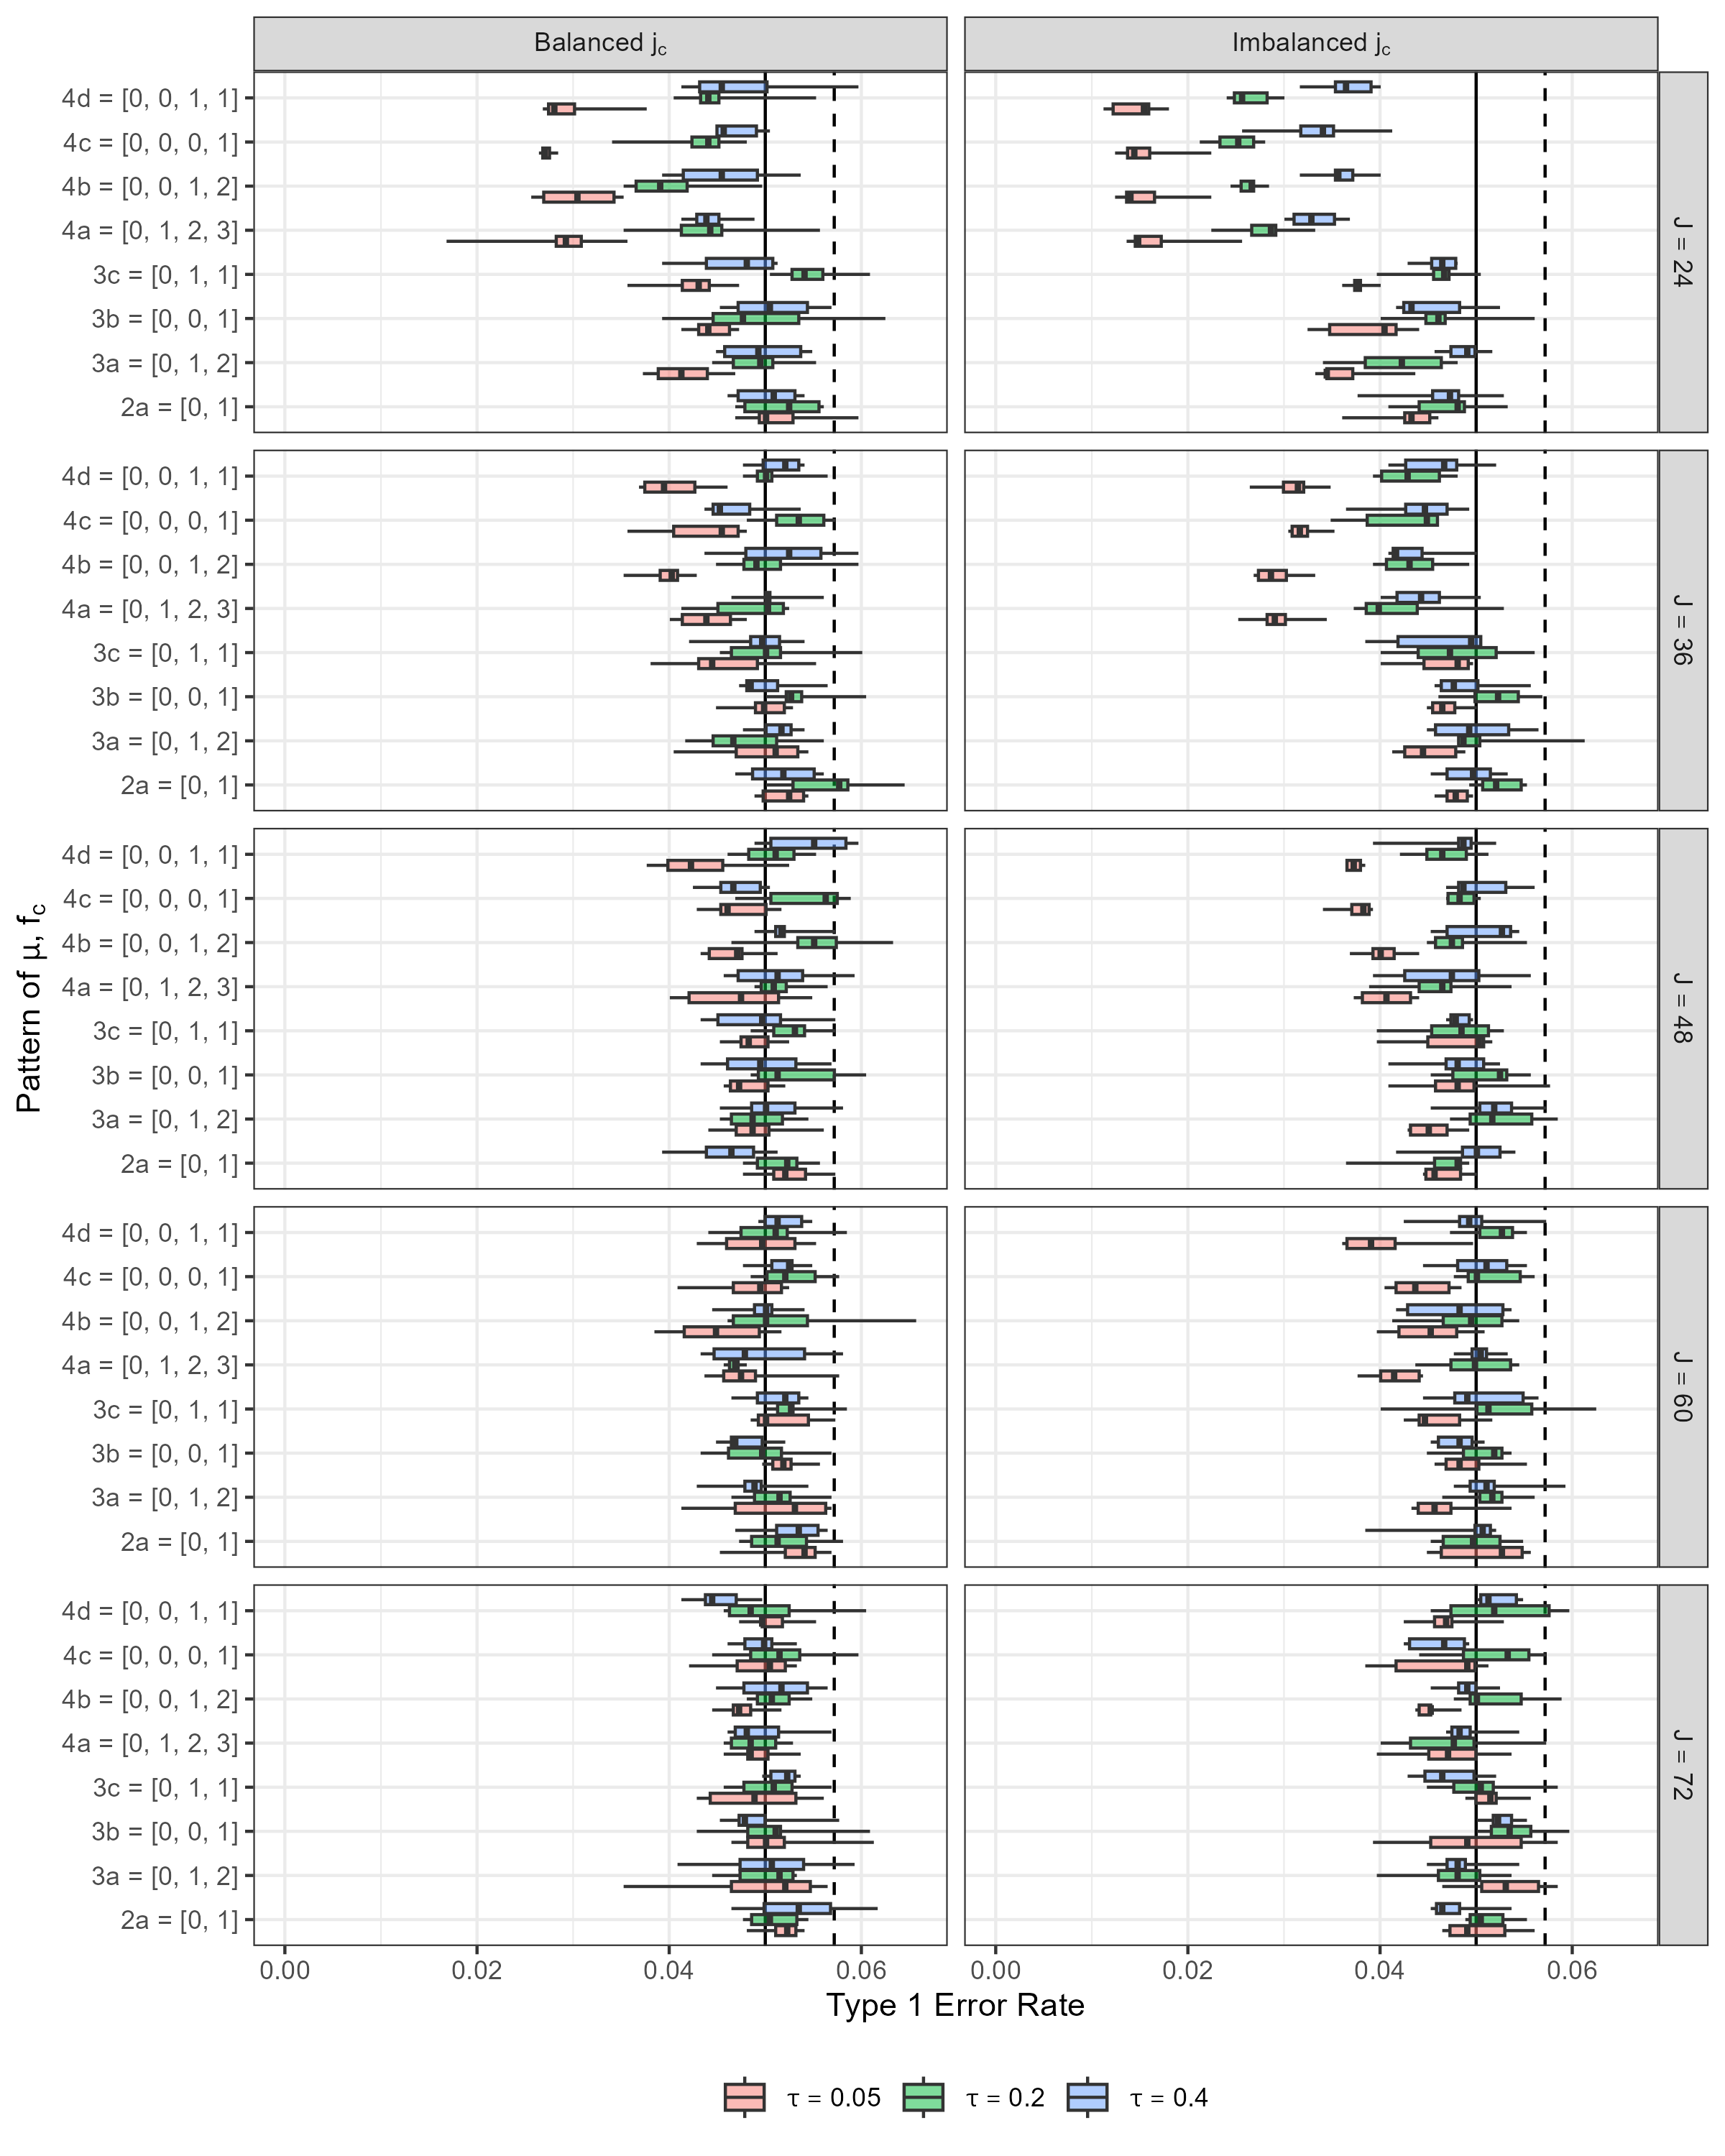
\includegraphics[width=\linewidth]{chapters/plots/type1error_bal_tau_all.png}\caption{Type I error by pattern type ($f_c$), the number of studies ($J$), between-study heterogeneity ($\tau$), and the balance of $j_c$ across categories (bal. $j_c$). The solid lines indicate $\alpha =.05$. The dashed lines indicate bounds for MCSE. \label{fig: type1error_bal_tau}}
    \vspace{-5pt}
\end{figure}







